% Paquets généraux
\documentclass[a4paper,12pt,titlepage,twoside]{article}
\usepackage[T1]{fontenc}
\usepackage[utf8]{inputenc}
\usepackage[french]{babel}
\usepackage{subcaption}
\addto\captionsfrench{%
  \renewcommand{\tablename}{Tableau}%
}
\usepackage[gen]{eurosym}
%\usepackage[dvips]{graphicx}
\usepackage{minted}
\usepackage{fancyhdr}
\usepackage{pdfpages} 
\usepackage{multido}
\usepackage{hyperref}
\usepackage{textcomp}
\usepackage{schemabloc}
%\usepackage[bitstream-charter]{mathdesign}
\usepackage{array}
\newcolumntype{P}[1]{>{\centering\arraybackslash}p{#1}}
\usepackage[shortlabels]{enumitem}
\usepackage[framemethod=TikZ]{mdframed}

\newcommand{\id}{30}
\newcommand{\nom}{Calculs d'hyperstatisme}
\newcommand{\sequence}{04}
\newcommand{\nomsequence}{Liaisons entre les solides}
\newcommand{\num}{03}
\newcommand{\type}{TD}
\newcommand{\descrip}{En appliquant les règles de la théorie des mécanisme, déterminer le degré d'hyperstatisme de plusieurs systèmes et proposer des solutions afin de diminuer ce degré}
\newcommand{\competences}{B2-12: Proposer une modélisation des liaisons avec leurs caractéristiques géométriques. \\ &  B2-13: Proposer un modèle cinématique paramétré à partir d'un système réel, d'une maquette numérique ou d'u \\ &  B2-17: Simplifier un modèle de mécanisme. \\ &  B2-18: Modifier un modèle pour le rendre isostatique.}
\newcommand{\nbcomp}{4}
\newcommand{\systemes}{E.P.A.S, Machine d'essai de traction}
\newcommand{\systemesnum}{14, 13}
\newcommand{\systemessansaccent}{E.P.A.S, Machine d'essai de traction}
\newcommand{\ilot}{3}
\newcommand{\ilotstr}{03}
\newcommand{\dossierilot}{\detokenize{Ilot_03 E.P.A.S, Machine d'essai de traction}}
\newcommand{\imageun}{EPAS}
\newcommand{\imagedeux}{Machine_dessai_de_traction}

%\usepackage{style}
\usepackage{bodegraph}
\usepackage{rpcinematik}
\usepackage[locale = FR]{siunitx}
\usepackage{caption}
\newcommand{\institute}{Lycée Dorian}
\usepackage{calc}

\usepackage{listings}
\usepackage{fancyvrb}
\usepackage{color}
\usepackage{xcolor}
\usepackage{colortbl}
\usepackage{helvet}
\usepackage[frenchmath]{newtxsf} % for sans serif symbols
\renewcommand{\familydefault}{\sfdefault}
%\usepackage{amsfonts}
%\usepackage{amsmath}
%\usepackage{lmodern}
\usepackage{mathastext}
%\usepackage{xspace}
\usepackage{varioref}
\usepackage{tabularx}
%\usepackage{floatflt}
\usepackage{graphics}
\usepackage{wrapfig}
\usepackage{textcomp}
\usepackage{tikz,tkz-tab}
\usepackage[european resistor, european voltage, european current]{circuitikz}
\usepackage{wrapfig}
\usepackage{gensymb}
\usepackage[percent]{overpic}
\usetikzlibrary{babel}
\usepackage{ifthen}
\usepackage{cancel}
\usepackage{etoolbox}
\usepackage{multirow}
%\usepackage{boxedminipage}
\definecolor{gris25}{gray}{0.75}
\definecolor{bleu}{RGB}{18,33,98}
\definecolor{bleuf}{RGB}{42,94,171}
\definecolor{bleuc}{RGB}{231,239,247}
\definecolor{bleum}{RGB}{160,195,226}
\definecolor{rougef}{RGB}{185,18,27}
\definecolor{rougec}{RGB}{255,188,204}%255,230,231
\definecolor{vertf}{RGB}{103,126,82}
\definecolor{vertc}{RGB}{220,255,191}
\definecolor{forestgreen}{rgb}{0.13,0.54,0.13}
\definecolor{blcr}{rgb}{0.59,0.69,0.84}
\definecolor{blfr}{rgb}{0.32,0.51,0.75}
\definecolor{orfr}{rgb}{0.90,0.42,0.15}
\definecolor{orcr}{rgb}{0.90,0.65,0.50}
\definecolor{orangef}{rgb}{0.659,0.269,0.072}
\definecolor{orange}{rgb}{0.58,0.35,0.063}
\definecolor{orangec}{rgb}{0.43,0.32,0.25}
\definecolor{rcorrect}{rgb}{0.6,0,0}
\definecolor{sequence}{rgb}{0.75,0.75,0.75}
\definecolor{competences}{rgb}{0.61,0.73,0.35}
\definecolor{rose}{HTML}{ff00ff}
\definecolor{grisf}{HTML}{222222}
\definecolor{grisc}{HTML}{636363}
\definecolor{normal}{HTML}{4087c4}
\definecolor{info}{HTML}{5bc0de}
\definecolor{success}{RGB}{92,184,92}
\definecolor{warning}{RGB}{240,173,78}
\definecolor{danger}{RGB}{217,83,79}
\hypersetup{                    % parametrage des hyperliens
    colorlinks=true,                % colorise les liens
    breaklinks=true,                % permet les retours à la ligne pour les liens trop longs
    urlcolor= blfr,                 % couleur des hyperliens
    linkcolor= orange,                % couleur des liens internes aux documents (index, figures, tableaux, equations,...)
    citecolor= forestgreen                % couleur des liens vers les references bibliographiques
    }

\newcolumntype{M}[1]{>{\centering\arraybackslash}m{#1}}
\definecolor{codegreen}{rgb}{0,0.6,0}
\definecolor{codegray}{rgb}{0.5,0.5,0.5}
\definecolor{codepurple}{rgb}{0.58,0,0.82}
\definecolor{backcolour}{rgb}{0.95,0.95,0.92}

\lstdefinestyle{mystyle}{
    backgroundcolor=\color{backcolour},   
    commentstyle=\color{codegreen},
    keywordstyle=\color{magenta},
    numberstyle=\tiny\color{codegray},
    stringstyle=\color{codepurple},
    basicstyle=\ttfamily\footnotesize,
    breakatwhitespace=false,         
    breaklines=true,                 
    captionpos=b,                    
    keepspaces=true,                 
    numbers=left,                    
    numbersep=5pt,                  
    showspaces=false,                
    showstringspaces=false,
    showtabs=false,                  
    tabsize=2
}

\lstset{style=mystyle}

% Mise en page
\pagestyle{fancy}

\setlength{\hoffset}{-18pt}
\setlength{\oddsidemargin}{0pt} 	% Marge gauche sur pages impaire2s
\setlength{\evensidemargin}{0pt} 	% Marge gauche sur pages paires
\setlength{\marginparwidth}{00pt} 	% Largeur de note dans la marge
\setlength{\headwidth}{481pt} 	 	% Largeur de la zone de tête (17cm)
\setlength{\textwidth}{481pt} 	 	% Largeu\textbf{r de la zone de texte (17cm)
\setlength{\voffset}{-18pt} 		% Bon pour DOS
\setlength{\marginparsep}{7pt}	 	% Séparation de la marge
\setlength{\topmargin}{-30pt} 		% Pas de marge en haut
\setlength{\headheight}{55pt} 		% Haut de page
\setlength{\headsep}{20pt} 		% Entre le haut de page et le texte
\setlength{\footskip}{30pt} 		% Bas de\textbf{ page + séparation
\setlength{\textheight}{700pt} 		% Hauteur de l'icone zone de texte (25cm)
\setlength\fboxrule{1 pt}
\renewcommand{\baselinestretch}{1}
\setcounter{tocdepth}{1}
\newcommand{\cadre}[2]
{\fbox{
  \begin{minipage}{#1\linewidth}
   \begin{center}
    #2\\
   \end{center}
  \end{minipage}
 }
}

\newcommand{\repon}[1]
{
~\ \\
\begin{tabular}{|m{\linewidth}|}
 \hline
\multido{}{#1}{\\ \hline}
\end{tabular}
}


\newcommand{\objectif}[1]{
\mdfsetup{%
frametitle={%
\tikz[baseline=(current bounding box.east),outer sep=0pt]
\node[anchor=east,rectangle,fill=bleum]
{\strut Objectif~};}}
\mdfsetup{innertopmargin=10pt,linecolor=bleum,%
linewidth=2pt,topline=true,%
frametitleaboveskip=\dimexpr-\ht\strutbox\relax
}
\begin{mdframed}[]\relax%
#1
\end{mdframed}}


\newcounter{num_quest} \setcounter{num_quest}{0}
\newcounter{num_rep} \setcounter{num_rep}{0}
\newcounter{num_cor} \setcounter{num_cor}{0}

\newcommand{\feuilleDR}[1]{
	\begin{tikzpicture}
		\draw[gray!30](0,0)grid[step=0.5cm](\linewidth,#1);
	\end{tikzpicture}
}

%\newcommand{\question}[1]{\refstepcounter{num_quest}\par
%~\ \\ \parbox[t][][t]{0.15\linewidth}{\textbf{Question \arabic{num_quest}}}\parbox[t][][t]{0.85\linewidth}{#1\label{q\the\value{num_quest}}}\par
%}

\newcommand{\question}[1]{\refstepcounter{num_quest}\par
~\ \\ \textbf{Question \arabic{num_quest} : }#1\label{q\the\value{num_quest}}\par
}

\newcommand{\posetafigure}[3]{
\begin{figure}[ht!]
 \begin{center}
  \includegraphics[width=#2\linewidth]{img/#1}
 \end{center}
 \caption{\label{#1} #3}
\end{figure}}

\newcommand{\goforum}{
\begin{figure}

\end{figure}
\begin{center}
 \includegraphics[width=0.7\linewidth]{../../../img/go_forum}
\end{center}
\label{go_forum}
\caption{J'pète les plombs}
\end{figure}}

\newcommand{\reponse}[4][1]
{\noindent
\parbox{\textwidth}{
\rule{\linewidth}{.5pt}\\
\textbf{Question\ifthenelse{#1>1}{s}{} \multido{}{#1}{%
\refstepcounter{num_rep}\ref{q\the\value{num_rep}} }:} ~\ \\
\ifdef{\public}{#3 \ifthenelse{#2>0}{~\ \\ 	\feuilleDR{#2}}}{#4}
}}

\newboolean{printdr}
\newboolean{printcor}
\setboolean{printdr}{false}
\setboolean{printcor}{false}

\newcommand{\reponseinfo}[2][1]
{\noindent
\rule{\linewidth}{.5pt}\\
\textbf{Question\ifthenelse{#1>1}{s}{} \multido{}{#1}{%
\refstepcounter{num_rep}\ref{q\the\value{num_rep}} }:} ~\ \\
\ifdef{\public}{\parbox{\textwidth}{\ifthenelse{#2>0}{~\ \\ 	\feuilleDR{#2}}}
\setboolean{printdr}{true}\setboolean{printcor}{false}}
{\setboolean{printdr}{false}\setboolean{printcor}{true}}
}

\makeatletter
\newcommand\modulo[2]{
    \newcounter{lastpagesujet}
	\setcounter{lastpagesujet}{#1}
    \divide\value{lastpagesujet} by #2
    \multiply\value{lastpagesujet} by #2
    \advance\value{lastpagesujet} by #2
    \advance\value{lastpagesujet} by 1\relax
    }
\makeatother

\newcommand{\finsujet}[1]
{
    \begin{center}
    \Large{FIN}
    \end{center}
        
    \ifthenelse{\equal{#1}{public}}{\def\public{}}{}

	\newpage

}

\newcommand{\debutcor}
{	
    \ifdef{\public}{
    	\modulo{\value{page}-1}{4}
		\whiledo{\value{page}<\value{lastpagesujet}}{~\ \newpage}
        \pagestyle{docreponse}
	}{\pagestyle{correction}}

    \ifdef{\public}{
        \begin{tikzpicture} 
            \draw (0,0) rectangle (2,2);
            \draw (0,0) -- (2,2);
            \draw (1.5,0.5) node {\large 20};
            \draw (2.5,0) rectangle (16,2);
            \draw (4.5,1.7) node {\large Commentaires:};
        \end{tikzpicture}
    }
    ~\ \\
}

%\newcommand{\repcarre}[2]
%{
%~\ \\
%\begin{tikzpicture}
%\draw [fill=white] (0,0) rectangle +(\linewidth,#1);
%\node[align=left] at (1.1,#2-0.3) {\textbf{Question #1:}};
%\end{tikzpicture}
%}

\newcommand{\titre}[1]
{\begin{center}
\cadre{0.8}{\huge #1} 
\end{center}
}


%Définition des torseurs :
\newcommand{\torseur}[2]{\left\{\mathcal{#1}_{#2} \right\}}
\newcommand{\torseurh}[3]{\left\{\genfrac{}{}{0pt}{0}{#1}{#2}\right\}_{#3}}
\newcommand{\torseurv}[8]{\left\{
\begin{matrix}
#1 & #4 \\ #2 & #5 \\ #3 &#6
\end{matrix}
\right\}_{{#7},{#8}}}

%Définition des torseurs :
%\newcommand{\torseur}[2]{\left \{\mbox{\relsize{2}{$\mathcal {#1}$}\relsize{-2}}\phantom{}_{\mbox{\scriptsize $#2$}} \right \}}
%\newcommand{\torseurh}[3]{\left\{\genfrac{}{}{0pt}{0}{#1}{#2}\right\}_{#3}}
%\newcommand{\torseurv}[8]{
%\left\{\begin{array}{@{}c|c@{}} #1 & #4 \\ #2 & #5 \\ #3 & #6 \end{array} \right\}_{#7,#8}
%}
\newcommand{\derivee}[2]{\left.\dfrac{\d #1}{\d t}\right|_{#2}}
\newcommand{\tripleint}{\int\!\!\!\!\!\int\!\!\!\!\!\int}

% Notation cinématique et statique
\newcommand{\cinematique}[2]{\mbox{#1}/\mbox{#2}}
\newcommand{\statique}[2]{\mbox{#1}\rightarrow\mbox{#2}}
\newcommand{\moment}[3]{\vv {#1}_{\scriptsize{#3}}(#2)}
\newcommand{\resultante}[2]{\vv {#1}_{\scriptsize{#2}}}


%Commande de base
\newcommand{\jo}{\left(j\omega\right)} % j \omega dans l'analyse fréquentielle
\newcommand{\tl}{\xrightarrow{\mathcal{L}}} % transformée de laplace sur fleche
\newcommand{\tli}{\xrightarrow{\mathcal{L}^{-1}}} % transformée inverse de laplace sur fleche
\renewcommand{\d}[1][]{\mathrm{d#1}}
\newcommand{\dd}[1][]{\mathrm{d#1}}
\newcommand{\vect}[2]{{#1}\wedge{#2}}
\newcommand{\base}[3]{(\vec #1,\vec #2,\vec #3)}
\newcommand{\vectbase}[4]{{\vphantom{\left| \begin{matrix}
#1\\#2\\#3 \end{matrix} \right|}}_{#4}{\left| \begin{matrix}
#1\\#2\\#3 \end{matrix} \right.}}
%Pour avoir les paragraphes sous la forme I, II, III
\renewcommand{\thesection}{\Roman{section}}
\setcounter{secnumdepth}{3}
\renewcommand{\Frlabelitemii}{$\bullet$}

% En tête et pied de page
\lhead{\nom}
\rhead{\includegraphics[width=2cm]{../../../img/logo}}
\lfoot{\auteurun,\ \auteurdeux}
\cfoot{Page \thepage}

\fancypagestyle{docreponse}{%
  \fancyhf{}
  \fancyhead[LO]{NOM Prénom: .............................}
  \rhead{\includegraphics[width=2cm]{../../../img/logo}\hspace{2pt}}
  \ifdef{\auteurdeux}{\lfoot{\auteurun,\ \auteurdeux}}{\lfoot{\auteurun}}
  \rfoot{\nom}
  \lfoot{Document réponse}
  \cfoot{Page \thepage}
   }

\fancypagestyle{correction}{%
  \fancyhf{}
  \lhead{\colorbox{danger}{\begin{minipage}{0.65\paperwidth} \textcolor{white}{\textbf{Correction}} \end{minipage}} }
  \rhead{\includegraphics[width=2cm]{../../../img/logo}}
  \lfoot{Renaud Costadoat, Françoise Puig}
  \rfoot{\colorbox{danger}{\begin{minipage}{0.3\paperwidth} \begin{flushright}\textcolor{white}{\textbf{Correction}}\end{flushright} \end{minipage}} }
  \cfoot{Page \thepage}
}

\fancypagestyle{correctioninfo}{%
  \fancyhf{}
  \lhead{\colorbox{danger}{\begin{minipage}{0.65\paperwidth} \textcolor{white}{\textbf{Correction}} \end{minipage}} }
  \rhead{\includegraphics[width=2cm]{../../../img/logo}}
  \lfoot{Renaud Costadoat, Juliette Genzmer}
  \rfoot{\colorbox{danger}{\begin{minipage}{0.6\paperwidth} \begin{flushright}\textcolor{white}{\textbf{Correction}}\end{flushright} \end{minipage}} }}

\renewcommand{\footrulewidth}{0.4pt}

\usepackage{eso-pic}
\newcommand{\BackgroundPic}{%
\put(0,0){%
\parbox[b][\paperheight]{\paperwidth}{%
\vfill
\begin{center}
\hspace{0.5cm}\vspace{0.5cm}
\includegraphics[width=\paperwidth,height=\paperheight,%
keepaspectratio]{../../../img/fond3}%
\end{center}
\vfill
}}}

\newcommand{\BackgroundPicdeux}{%
\put(25,-30){%
\parbox[b][\paperheight]{\paperwidth}{%
\vfill
\begin{center}
\includegraphics[width=\paperwidth,height=\paperheight,%
keepaspectratio]{../../../img/fond4}%
\end{center}
\vfill
}}}

\begin{document}

\pagestyle{empty}

\AddToShipoutPicture*{\BackgroundPic}

\includegraphics[width=2cm]{../../../img/logo}

\Huge{DS \numero - \sujet}

\vspace{1cm}

\ifdef{\prive}{\begin{center}\colorbox{danger}{\Huge{Avec Correction}}\end{center}}{}

\begin{center}
\centering\huge{PTSI}
\end{center}

\vspace{2cm}


\begin{center}
\centering\Large{\jour}
\end{center}

\vspace{2cm}

\normalsize

\tableofcontents

\newpage

\AddToShipoutPicture{\BackgroundPicdeux}

\pagestyle{fancy}

\begin{center}
\Huge \sujet
\end{center}


\normalsize


\section{Problématique et objectif}

En culture hors-sol (figure \ref{fig01}), il faut constamment déplacer les pots pour profiter de la lumière, pour regrouper les cultures, isoler celles qui posent problème, ... Ce travail est pénible physiquement et les pépiniéristes peinent à trouver de la main d'\oe uvre pour réaliser ces tâches quotidiennes difficiles.

\begin{figure}[ht!]
\begin{minipage}{0.46\linewidth}
\begin{center}
 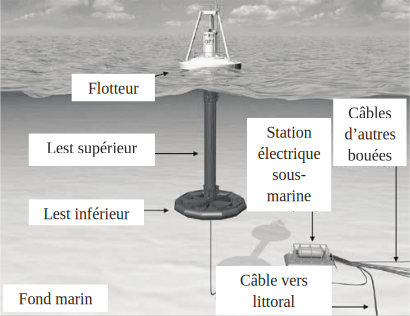
\includegraphics[width=0.8\linewidth]{img/fig01}
\end{center}
\caption{Exemple de culture hors-sol}
\label{fig01}
\end{minipage}
\hfill
\begin{minipage}{0.46\linewidth}
\begin{center}
 \includegraphics[width=0.8\linewidth]{img/fig02}
\end{center}
\caption{Robot TROOPER de la société INSTAR ROBOTICS}
\label{fig02}
\end{minipage}
\end{figure}

La Startup INSTAR ROBOTICS, spécialisée dans le développement de robots d'assistance, a conçu le robot TROOPER qui permet de répondre à ce besoin (figure \ref{fig02}).

L'objectif du travail proposé dans cette épreuve est de justifier les solutions techniques retenues par la société INSTAR ROBOTICS dans le but de respecter le cahier des charges élaboré en partenariat avec des pépiniéristes.

\section{Cahier des charges}

Les spécifications que doit respecter le robot sont directement liées aux contraintes imposées par la culture hors-sol.

Une des contraintes majeures est la vitesse à laquelle le robot doit se déplacer et réaliser les opérations de prise/dépose de pots afin d'être si possible aussi rapide qu'une personne.

Un exemple de tâche à réaliser consiste à déplacer 4 rangées de 6 pots d'une zone à une autre. Le robot doit prendre les 6 pots de la rangée 1 de la zone 1, puis les déplacer dans la rangée 1 de la zone 2, de même pour les autres rangées.

On note $T_p$ le temps de prise d'une rangée de 6 pots, égal au temps de dépose (ce temps inclut toutes les man\oe uvres et est estimé à 30 s). On suppose que le robot se déplace à la vitesse constante $V$ en ligne droite sur une distance $L=10m$ séparant les rangées de chaque zone (figure \ref{fig03}). La distance entre deux rangées d'une zone est notée $\ell=50cm$.

\begin{figure}[ht!]
\begin{center}
 \includegraphics[width=0.8\linewidth]{img/fig03}
\end{center}
\caption{Tâche à effectuer par le robot}
\label{fig03}
\end{figure}

Un employé qui utilise un chariot à pousser (pour déplacer 6 pots à chaque fois) met un temps total $T_m$ pour réaliser cette tâche de repositionnement de 4 rangées de pots.

\question{Déterminer la vitesse $V$, supposée constante, à laquelle doit se déplacer le robot en ligne droite pour réaliser la tâche au maximum en $T_m$ secondes en fonction de $L$, $\ell$, $T_m$ et $T_p$. Faire l'application numérique pour une durée $T_m$ de 320 secondes.}

Les autres éléments du cahier des charges pourraient être justifiés de la même manière. Le diagramme des exigences de la figure \ref{fig04} liste les éléments principaux utiles pour le dimensionnement du robot.

Le robot est constitué de plusieurs chaînes d'énergie et d'information. Nous analyserons dans un premier temps les chaînes d'énergie et d'information relatives au déplacement du robot, puis, dans un second temps, celles relatives à la prise et dépose des pots.

Pour se déplacer, le robot utilise deux roues motorisées indépendantes à l'avant et deux roues folles à l'arrière. Le robot embarque une batterie pouvant délivrer jusqu'à 100 Volts. Une carte de commande dédiée à chaque moteur utilise l'information d'un codeur incrémental monté sur chaque axe moteur pour donner des ordres au hacheur pilotant ce même moteur. Un réducteur permet d'adapater la vitesse de rotation du moteur pour la transmettre à la roue. Pour permettre au robot de se diriger correctement, un dispositif LIDAR (Laser Imaging Detection And Ranging : émetteur/récepteur infrarouge) fournit des informations sur l'environnement à un micro-ordinateur qui se charge d'envoyer des consignes aux cartes de commande des moteurs. L'utilisateur peut communiquer avec le robot à l'aide d'une tablette en Bluetooth.

\question{À l'aide des informations ci-dessus, compléter les chaînes d'énergie et d'information pour le déplacement du robot.}

\newpage

\begin{figure}[ht!]
\begin{center}
 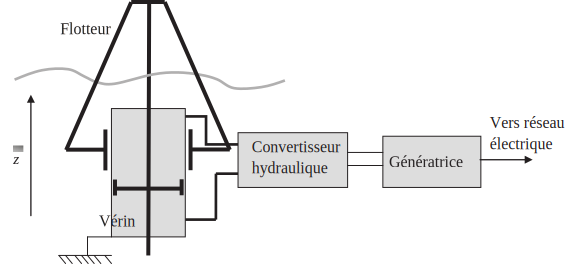
\includegraphics[width=0.8\linewidth]{img/fig04}
\end{center}
\caption{Diagramme des exigences du robot Trooper}
\label{fig04}
\end{figure}

\vspace{-1cm}

\section{Déplacement du robot}

Nous allons montrer tout d'abord la nécessité d'asservir en vitesse les moteurs pour assurer un déplacement correct du robot.

\subsection{Nécessité d'un asservissement en vitesse}

Chaque roue motorisée du robot a pour rayon $r=15cm$ et le rapport de réduction du réducteur associé à chaque moteur vaut $k_r=\dfrac{1}{40}$.

Les caractéristiques d'un moteur sont :
\begin{itemize}
 \item $J_m=3,4\cdot 10^{-3} kg\cdot m^2$ moment d'inertie de l'ensemble motoréducteur ramené sur l'arbre moteur,
 \item $k_m=0,2Nm\cdot A^{-1}$ constante de couple (égale à la constante de vitesse),
 \item $R_m=1\Omega$ résistance interne du moteur,
 \item vitesse maximale du moteur égale à $3000tr\cdot min^{-1}$.
\end{itemize}

\question{Vérifier que les éléments choisis permettent de respecter le critère de vitesse maximale défini dans le diagramme des exigences.}

\begin{figure}[ht!]
\begin{minipage}{0.6\linewidth}
On souhaite que le robot se déplace selon une loi trapèze de vitesse avec $V_{max}$ la vitesse maximale du robot (du diagramme des exigences) pour parcourir une distance
$D=10m$. On donne le temps total $T=10s$ et on cherche la durée d'accélération égale à la durée de décélération $\delta t$. Pour la question suivante, on suppose, de manière simplifiée, que le robot suit parfaitement cette consigne.
\end{minipage}
\hfill
\begin{minipage}{0.36\linewidth}
\begin{center}
 \includegraphics[width=0.9\linewidth]{img/fig04b}
\end{center}
\end{minipage}
\end{figure}

\question{Déterminer l'expression du temps $\delta t$ pour respecter le déplacement souhaité en fonction de $D$, $T$ et $V_{max}$. Faire l'application numérique.}

~\

On suppose que les deux moteurs sont identiques. Les équations qui caractérisent le comportement en ligne droite du robot sont les suivantes :
\begin{eqnarray}
u_m(t)=R_mi_m(t)+k_m\omega_m(t)\\
2C_m(t)-C_r(t)=J\dfrac{d\omega_m(t)}{dt}\\
C_m(t)=k_mi_m(t)\\
v(t)=k_t\omega_m(t)
\end{eqnarray}

Avec $\omega_m(t)$ est la vitesse angulaire d'un moteur, $u_m(t)$ la tension de commande d'un moteur, $i_m(t)$ le courant traversant chaque moteur et $C_m(t)$ le couple exercé par un moteur.

$C_r(t)$ est un couple résistant global supposé nul dans un premier temps pour Q5 et Q6. $J$ est le moment d'inertie équivalent de l'ensemble en mouvement ramené sur un arbre moteur. $v(t)$ est la vitesse du robot en ligne droite par rapport au sol.

\question{Déterminer l'équation différentielle vérifiée par $v(t)$ avec $u_m(t)$ comme entrée. Vérifier que $v(t)=\alpha_0(t-\tau_m+\tau_m e^{\frac{-t}{\tau_m}})$ est solution de l'équation différentielle pour une consigne de tension $u_m(t)=\frac{u_0}{\delta t}.t.u(t)$, où $u(t)$ est un échelon unitaire. On suppose que $v(0)=0$. On donnera l'expression de $\alpha_0$ et $\tau_m$ en fonction de $u_0$, $\delta t$ et des constantes intervenant dans les équations du moteur.}

~\

La figure \ref{fig05} montre la réponse du robot à une tension de commande en trapèze. La courbe de vitesse simulée est tracée ainsi que la courbe de vitesse de consigne fournie.

\question{En s'aidant de l'expression de la vitesse donnée précédemment, estimer la valeur de $\tau_m$ à partir de la courbe de vitesse réelle. Faire apparaître le tracé sur la figure du Document Réponse.}

~\

Au regard des simulations effectuées, on constate qu'on peut confondre la vitesse de consigne avec la vitesse simulée et ainsi travailler directement avec le profil de vitesse de consigne pour des études cinématiques.

Le robot évolue sur un terrain souvent boueux et accidenté, ce qui engendre des perturbations sur les roues, le robot ne se déplace alors plus à la vitesse souhaitée. De plus, pour des courants trop faibles, les roues ne tournent pas à cause des frottements. La vitesse de déplacement du robot est donc asservie à une vitesse de consigne notée $v_c(t)$.

\newpage

\begin{figure}[ht!]
\begin{center}
 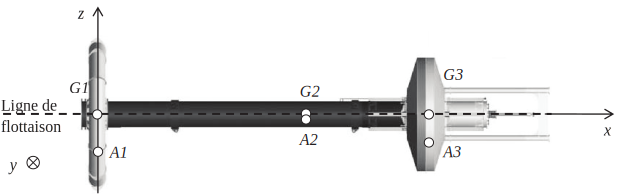
\includegraphics[width=0.7\linewidth]{img/fig05}
\end{center}
\caption{Simulation du déplacement du robot en réponse à une consigne en trapèze}
\label{fig05}
\end{figure}

Un adaptateur de gain $K_a$ convertit la consigne $v_c(t)(m\cdot s^{-1})$ en une valeur numérique notée $n_c(t)$.

Cette valeur numérique est comparée à l'image $n_m(t)$ de la vitesse de rotation des moteurs $\omega_m(t)$ déterminée à l'aide d'un codeur incrémental de gain $K_c$. Celui-ci délivre 628 informations (ou inc) par tour de moteur.

L'écart $\varepsilon(t)$ ainsi formé est adapté par un ensemble correcteur amplificateur dont la fonction de transfert sera notée $C(p)$ pour fournir la tension d'alimentation $u_m(t)$ aux moteurs.

La vitesse de rotation des moteurs $\omega_m(t)$ est adaptée par l'ensemble réducteur-roue de gain $k_t$ pour obtenir la vitesse $v(t)$ de déplacement du robot.

Des perturbations sur les moteurs sont prises en compte sous la forme d'un couple résistant noté $C_r(t)$.

\question{À partir des équations (1), (2) et (3), déterminer la relation $\Omega_m(p)=H_m(p).U_m (p)+H_r(p).C_r(p)$ où l'on précisera l'expression de $H_m(p)$ et $H_r(p)$ sous forme canonique.}

\question{Compléter le schéma-bloc de l'asservissement de vitesse linéaire du robot en utilisant les indications précédentes. Préciser la valeur numérique de $K_c$ en $inc/rad$. Donner l'expression de $K_a$ permettant d'assurer un asservissement correct.}

~\

On choisit de prendre un correcteur de la forme $C(p)=K_p\dfrac{1+\tau_i p}{\tau_i p}$.

\question{Nommer le correcteur et justifier le choix de ce correcteur.}

~\

On prend pour valeur de $\tau_i$ la valeur de la constante de temps du moteur : $\tau_i =\tau_m$.

\newpage

Compte tenu de la valeur choisie pour $K_a$, le schéma-bloc de l'asservissement de vitesse peut être mis sous forme de schéma-bloc à retour unitaire dont la Fonction de Transfert en Boucle Ouverte est :
\begin{center}
	$FTBO(p)=C(p)\dfrac{K_mK_c}{1+\tau_mp}$
\end{center}
avec $K_mK_c=500inc\cdot s^{-1}\cdot V^{-1}$ et $\tau_m=0,1s$.

\question{Déterminer la valeur de $K_p$ pour que le temps de réponse à 5\% en boucle fermée soit égal à 0,3 s.}

~\

La figure \ref{fig06} représente la réponse du robot pour une consigne en trapèze en utilisant un correcteur bien réglé et en prenant en compte des perturbations de type \textbf{frottement sec}. Pour prendre en compte le couple $C_r$ dans la simulation, un bloc non-linéaire a été introduit dans le schéma-bloc pour aboutir à cette réponse.

\begin{figure}[ht!]
\begin{center}
 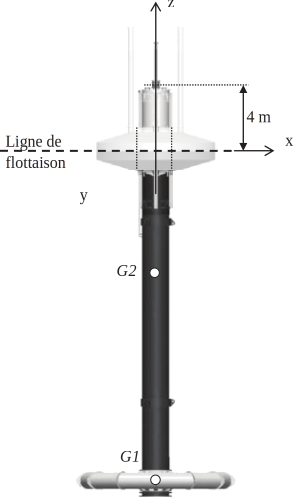
\includegraphics[width=0.7\linewidth]{img/fig06}
\end{center}
\caption{Simulation de la vitesse du robot asservi en réponse à une consigne en trapèze}
\label{fig06}
\end{figure}

\question{Entourer sur la courbe la zone qui montre que la perturbation a été prise en compte. Préciser quelle non-linéarité (à choisir parmi saturation, seuil, hystérésis) a été retenue. Conclure sur la pertinence de l'asservissement de vitesse mis en place vis-à-vis des performances attendues.}

\subsection{Comportement en pente}

La motorisation retenue permet de déplacer le robot sur sol horizontal même en présence d'une perturbation de type frottement sec. Il faut cependant vérifier qu'elle permet également au robot de gravir des pentes comme indiqué dans le diagramme des exigences (Id 1.2.1), ce qui correspond à une perturbation supplémentaire.

On se place dans le cas où le robot supporte 6 pots de masse $m=10kg$ chacun. On note $M=60kg$ la masse du robot. On associe au sol le repère $(O, \vec{x}, \vec{y}_0, \vec{z}_0)$ incliné d'un angle $\alpha=(\vec{y},\vec{y}_0)=(\vec{z},\vec{z}_0)$
constant par rapport à l'horizontale.

Le robot se déplace en ligne droite selon  $(O, \vec{y}_0)$ à la vitesse $v(t)$, en phase de montée. On note $C_m(t)$ le couple appliqué par chaque moteur pour faire avancer le robot. Les liaisons sont toutes supposées parfaites énergétiquement et le robot roule sans glisser sur le sol (figure \ref{fig07}).

\newpage

\begin{figure}[ht!]
\begin{center}
 \includegraphics[width=0.7\linewidth]{img/fig07}
\end{center}
\caption{Paramétrage pour l'étude en pente du robot (représenté sans les pots)}
\label{fig07}
\end{figure}

On rappelle que $v(t)=k_t \omega_m(t)$. On négligera l'inertie des réducteurs et des roues.

Une application du théorème de l'énergie cinétique au robot en mouvement, a permis d'écrire l'équation qui décrit le mouvement du robot en pente suivante :\\ 
$M_{eq}\dfrac{dv(t)}{dt}=\dfrac{1}{r_{eq}}C_m(t)-F_{r,eq}$.

Avec $M_{eq}=M+6m$, $r_{eq}=\dfrac{k_t}{2}$ et $F_{r,eq}=(M+6m)g\sin\alpha$.

Pour vérifier le dimensionnement des moteurs, on utilise les valeurs suivantes pour les constantes précédentes : $M_{eq}\approx 120 kg$, $r_{eq}\approx 2\cdot 10^{-3} m$, $F_{r,eq}\approx 200 N$.

On considère à nouveau la loi de pilotage définie précédemment sous forme de trapèze avec $V_{max} = 1,1 m\cdot s^{-1}$, $\delta t=1s$ et $T=10s$.

\question{Tracer l'évolution de $C_m(t)$ au cours du temps compte tenu de l'évolution souhaitée de $v(t)$. Préciser les valeurs caractéristiques sous forme littérale, puis numérique.}

\question{À l'aide des équations du moteur, déterminer le couple maximal développé par un moteur lorsqu'il est alimenté sous $100V$. Vérifier alors que la motorisation est adaptée à une montée en pente du robot.}

\subsection{Pilotage du robot}

La société qui développe le robot propose une application sur tablette qui permet, soit de piloter manuellement le robot, soit de lui faire réaliser des tâches automatisées. 

Pour cela, le robot utilise le LIDAR qui détermine la position des pots environnants par rapport au robot.

Pour pouvoir se déplacer dans toutes les directions, il faut contrôler le comportement du robot et notamment définir correctement les consignes de vitesse de chaque roue motorisée.

Le paramétrage du robot est donné sur la figure \ref{fig08}.

La distance séparant les centres des roues motrices au point O est notée $e=AO=OB$. 

Le rayon d'une roue est noté $r$.

On suppose que le mouvement du robot noté 1 par rapport au sol noté 0 est défini par le torseur cinématique $\left\{V_{1/0}\right\}=\left\{\begin{array}{c}\dot{\theta}\vec{z}\\V\vec{y}_1\end{array}\right\}$. On note A' le point de contact de la roue gauche avec le sol et B' le point de contact de la roue droite avec le sol. On note $\omega_d$ (respectivement $\omega_g$) les vitesses de rotation des roues droite (notée d) et gauche (notée g) par rapport au robot 1.

\begin{figure}[ht!]
\begin{center}
 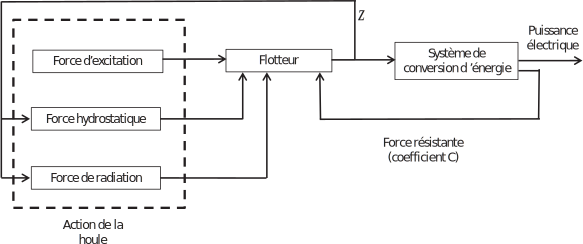
\includegraphics[width=0.7\linewidth]{img/fig08}
\end{center}
\caption{Paramétrage du robot en virage}
\label{fig08}
\end{figure}

\question{Déterminer la vitesse $\vec{V}(A'\in g/0)$ en fonction de $V$, $\omega_g$, $\dot{\theta}$, $e$ et $r$. De même, sans détailler les calculs, donner l'expression de $\vec{V}(B'\in d/0)$ en fonction de $V$, $\omega_d$, $\dot{\theta}$, $e$ et $r$.}

\question{En utilisant l'hypothèse de roulement sans glissement en A' et en B', montrer que $\dot{\theta}=C_1(\omega_g-\omega_d)$ et $V=-C_2(\omega_d+\omega_g)$ où $C_1$ et $C_2$ sont des constantes positives à exprimer en fonction des données.}

~\ \\ ~\

Il existe deux modes de pilotage manuel (figure \ref{fig09}).

Dans le premier cas (pilotage direct), on contrôle la vitesse de chaque roue grâce à deux curseurs : le robot est difficile à déplacer.

Dans le second cas (pilotage indirect), un premier curseur permet de spécifier la vitesse du centre du robot entre $-V_c$ et $+V_c$ et un autre curseur permet de contrôler la vitesse de rotation du robot $\dot{\theta}$ entre $-\omega_c$ et $+\omega_c$ (rotation autour de l'axe $(O,\vec{z})$). En utilisant le curseur de vitesse d'avance uniquement on peut faire avancer ou reculer le robot. Si on utilise uniquement le deuxième curseur (vitesse de rotation du robot), on peut le faire tourner sur place vers la gauche ou vers la droite.

\newpage

\begin{figure}[ht!]
\begin{center}
 \includegraphics[width=0.7\linewidth]{img/fig09}
\end{center}
\caption{Application de pilotage du robot}
\label{fig09}
\end{figure}

\question{Indiquer les consignes qu'il faut imposer à chaque roue pour obtenir les quatre déplacements souhaités en fonction de $C_1$, $C_2$, $V_c$ et $\omega_c$.}

~\

%Le LIDAR donne la distance qui sépare un pot du robot ainsi que l'angle par rapport à la direction d'avance du robot. Avec ces informations, pour aller récupérer un pot, il suffit de faire tourner le robot sur lui-même (en faisant tourner une roue dans un sens et l'autre dans le sens inverse avec $V=0$) d'un angle $\theta_c$ pendant un temps $t_c$ à une vitesse angulaire donnée $\omega_c$ pour l'orienter correctement (pour ce déplacement, on notera $\pm \omega_1$ la vitesse de rotation des roues). Puis, on fait avancer le robot vers le pot en ligne droite (pour ce déplacement, les vitesses des roues sont notées $\pm \omega_2$). Lorsque la distance $\ell$ renvoyée par le LIDAR est inférieure ou égale à une distance donnée $\ell_c$, le robot s'arrête pour pouvoir prendre le pot.

%\question{Compléter les info-bulles du diagramme d'état qui décrit le comportement du robot avec les valeurs de $\omega_d$ et $\omega_g$, ainsi que les deux transitions manquantes.}

\section{Prise des pots}

La deuxième fonction principale du robot est de pouvoir prendre et déposer des pots d'une taille donnée. L'objectif de cette partie est d'analyser le mécanisme de prise et dépose des pots.

\subsection{Solution brevetée}

La société INSTAR ROBOTICS a déposé un brevet concernant la solution permettant de prendre les pots (figure \ref{fig10}). Cette solution utilise deux moteurs, l'un pour rapprocher les bras et l'autre pour les lever et placer un pot dans une zone pouvant contenir 6 pots (magasin). Des capteurs permettent de détecter lorsque les bras sont en position ouverte (bras complètement écartés) ou en position fermée (pinces en contact l'une avec l'autre). De même, des capteurs permettent de détecter la position haute et la position basse des bras. En position haute, il suffit d'ouvrir les bras pour que le pot soit bien placé dans la zone de stockage des pots. Pour détecter qu'il est possible de lever un pot, le courant $i$ parcourant les moteurs est utilisé. S'il dépasse une valeur $i_0$, cela veut dire que le pot est serré suffisamment fort entre les deux mains et qu'il est possible de le lever.

\newpage

\begin{figure}[ht!]
\begin{center}
 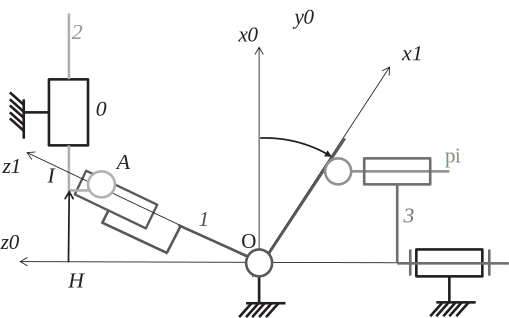
\includegraphics[width=0.65\linewidth]{img/fig10}
\end{center}
\caption{Description du mouvement bras}
\label{fig10}
\end{figure}

La zone de stockage des pots est mise en mouvement par un moteur asservi en position qui réalise 1/6e de tour lorsqu'un pot est correctement positionné.

\question{Proposer une solution mécanique (uniquement le nom de la solution) permettant de réaliser 1/6e de tour sans avoir besoin d'asservir le moteur.}

~\

La solution retenue pour prendre les pots est donnée sur le schéma cinématique de la figure \ref{fig11}.

\question{Indiquer quel moteur entraîne le rapprochement des bras ($M_1$ ou $M_2$) et celui qui permet de soulever le pot. Justifier pourquoi les " mains " se déplacent toujours parallèlement au sol et ce que cela implique sur les pots.}

\begin{figure}[ht!]
\begin{center}
 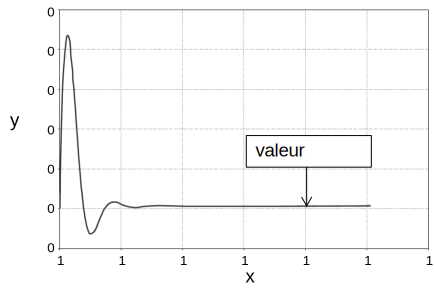
\includegraphics[width=0.9\linewidth]{img/fig11}
\end{center}
\caption{Cinématique du système de prise des pots}
\label{fig11}
\end{figure}

\newpage

Le mouvement entre chaque crémaillère et le châssis est réalisé par quatre liaisons pivot glissant (figure \ref{fig12}).

\begin{figure}[ht!]
\begin{center}
 \includegraphics[width=0.6\linewidth]{img/fig12}
\end{center}
\caption{Modélisation simplifiée des liaisons entre la crémaillère et le châssis}
\label{fig12}
\end{figure}

\question{Déterminer le degré d'hyperstatisme (modèle spatial) associé à cet ensemble de liaisons (figure \ref{fig12}) et indiquer la conséquence d'une telle solution.}

~\

Le mouvement d'élévation d'une main est réalisé par un mécanisme qui peut être modélisé comme sur la figure \ref{fig13}.

\begin{figure}[ht!]
\begin{center}
 \includegraphics[width=0.6\linewidth]{img/fig13}
\end{center}
\caption{Modélisation simplifiée du mécanisme d'élévation}
\label{fig13}
\end{figure}

\question{Proposer une modélisation isostatique sans changer le nombre de liaisons du modèle de la figure \ref{fig13}. Faire le calcul du degré d'hyperstatisme de la solution proposée en précisant bien les mobilités, en considérant le modèle spatial. Réaliser un schéma cinématique dans le plan $(\vec{y}O\vec{z})$ de la solution isostatique.}

~\

Les motoréducteurs retenus pour prendre et soulever les pots délivrent un couple maximal de $12 Nm$.

Leur vitesse maximale est égale à $200tr\cdot min^{-1}$. Le pignon du dispositif pignon-crémaillère possède $Z = 20 dents$. Le pas entre les dents sur la crémaillère est égal à $p=10 mm$. Le rayon du pignon vaut ainsi $r_p=\dfrac{Zp}{2\pi}$. On suppose que les pinces sont en contact ponctuel avec un pot de masse $m=10 kg$ sans contact avec le sol.

L'accélération de la pesanteur est notée $-g\cdot\vec{z}$ avec $g=10m\cdot s^{-2}$.

~\

On note :
\begin{itemize}
 \item $\left\{T_{main1\rightarrow pot}\right\}=\left\{\begin{array}{c}
 N_1\vec{x}+T_1\vec{z}\\ \vec{0} \end{array} \right\}_{I_1}$, l'action mécanique de la main 1 sur le pot,
 \item $\left\{T_{main2\rightarrow pot}\right\}=\left\{\begin{array}{c}
 -N_2\vec{x}+T_2\vec{z}\\ \vec{0} \end{array} \right\}_{I_2}$, l'action mécanique de la main 2 sur le pot.
\end{itemize}

Le coefficient de frottement entre les pinces et le pot est pris égal à $f_p=0,3$. Ainsi, à la limite du glissement, on pourra écrire $T_i=f_pN_i$ (i = 1 ou i = 2).
 
\question{En isolant le pot, déterminer les composantes normales minimales $N_1$ et $N_2$ à appliquer de chaque côté du pot.}

~\

L'action mécanique d'une crémaillère sur le pignon est simplement modélisée par un glisseur de résultante portée par $\vec{x}$ appliquée en un point $I_{ci}$(i = 1 ou i = 2), comme sur la figure \ref{fig14}. A ces actions s'ajoute le couple moteur d'axe $(O,\vec{z})$. On suppose l'ensemble à l'équilibre.

\begin{figure}[ht!]
\begin{center}
 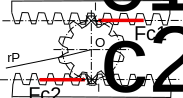
\includegraphics[width=0.6\linewidth]{img/fig14}
\end{center}
\caption{Paramétrage pignon crémaillère}
\label{fig14}
\end{figure}

\question{Isoler le pignon et en déduire $C_0$ en fonction de $r_p$ et de $F_{c1}$.}

\question{Isoler l'ensemble $\sum_1=\left\{\textrm{crémaillère 1 + biellette 1 + noyau cannelé 1 + main 1}\right\}$, soumis aux actions mécaniques extérieures suivantes : action du pignon sur la crémaillère $F_{c1}\vec{x}$, l'action du pot sur la main en $I_1$, et action du châssis. En déduire que le couple minimal vaut $C=r_0mg$ en donnant l'expression de $r_0$ en fonction de $r_p$ et $f_p$. Sachant que $r_0=106mm$, vérifier si le motoréducteur retenu est satisfaisant.}

\subsection{Basculement}

Lors de la prise d'un pot, il est possible que le robot bascule. Pour éviter ce problème, la batterie a été placée à l'arrière pour décaler le centre de gravité. L'objectif des questions suivantes est de déterminer la masse d'un pot provoquant le basculement du robot.

\question{Décrire la situation la plus défavorable en fonction de la position des bras et du nombre de pots sur le robot.}

On utilise le paramétrage de la figure \ref{fig14}. On note $M=60kg$ la masse du robot à vide et $m=10kg$ la masse d'un pot. Le centre de gravité du robot à vide est noté G et le centre de gravité du pot est noté P.

~\

Le problème est supposé symétrique et plan, ce qui permet de considérer un demi-robot, de masse $M/2$, en contact en deux points C et D avec le sol et qui porte un demi-pot de masse $m/2$.

\newpage

\begin{figure}[ht!]
\begin{center}
 \includegraphics[width=0.7\linewidth]{img/fig15}
\end{center}
\caption{Paramétrage pour l'étude du basculement}
\label{fig15}
\end{figure}

On suppose que les actions mécaniques en C et D sont des glisseurs de résultantes :
\begin{center}
$\vec{F}(\textrm{sol}\rightarrow \textrm{roue\ arriere})=N_C\vec{z}+T_C\vec{y}$ et $\vec{F}(\textrm{sol}\rightarrow \textrm{roue\ avant})=N_D\vec{z}+T_D\vec{y}$
\end{center}

\question{En précisant le système isolé et en choisissant une seule équation issue du principe fondamental de la statique, déterminer l'expression de l'effort normal sur la roue arrière $N_C$ en fonction de $g$, $a$, $b$, $c$, $M$ et $m$.}

~\

Le basculement intervient lorsque $N_c=0$

\question{En déduire la masse maximale d'un pot qui entraîne ce basculement. Conclure vis-à-vis du diagramme des exigences.}

%On note $\gamma$ l'accélération longitudinale du robot, $C_{mr}$ le couple induit par les motoréducteurs sur les roues avant, $r$ le rayon des roues avant, $f=0,5$ le facteur de frottement des roues sur le sol. On néglige le moment d'inertie des roues selon leur axe de rotation.

%Le problème est toujours supposé symétrique et plan, ce qui permet de considérer un demi-robot, de masse $M/2$, en contact en deux points C et D avec le sol. On se place dans le cas où le robot ne porte pas de pot. On peut montrer que :

%\begin{eqnarray}
%\frac{M}{2}\gamma=T_C+T_D \\
%\frac{M}{2}g=N_C+N_D \\
%-bN_C+(b-a)\frac{M}{2}g=-h\frac{M}{2}\gamma
%\end{eqnarray}

%\question{Indiquer quel théorème a été utilisé pour obtenir chaque équation (nom du théorème, point,projection).}

%\question{Sachant que seule la roue avant est motrice (contact en $D$), en déduire l'expression littérale de $T_D$.}

%On retient une accélération égale à celle spécifiée en deuxième partie : $\gamma=1,1 m\cdot s^{-2}$.

%\question{Déterminer numériquement $T_D$ puis $N_D$ pour les valeurs retenues et indiquer si la roue avant glisse ou non dans cette situation.}

%\question{En se plaçant à la limite du glissement en $D$, donner l'expression et la valeur de l'accélération maximale qu'il est possible d'avoir pour éviter le glissement. En déduire la durée de la phase d'accélération permettant d'atteindre la vitesse maximale dans ces conditions.}

%\section{Synthèse}

%Le diagramme d'état donné dans le Document Réponse propose une description possible des différentes tâches réalisées par le robot pour la configuration décrite au départ (Q1). Pendant tout le fonctionnement, le LIDAR fournit la distance entre le robot et le pot à prendre. Au départ, l'utilisateur amène le robot manuellement en position initiale (les bras sont en bas et écartés). Ensuite, le bouton start est actionné, le cycle peut commencer. On rappelle que la description des capteurs à disposition est donnée dans le paragraphe introductif de la sous-partie IV.1.

%\question{En vous aidant des informations données tout au long du sujet, compléter les états à l'aide des propositions suivantes : " rapprochement des bras ", " écartement des bras ", " élévation des bras ", " abaissement des bras " et " rotation magasin de 60\degree".}

%\question{Compléter les 6 transitions en pointillées du diagramme d'état représentant l'état composite " prise d'un pot ". Vous utiliserez notamment les évènements " haut ", " bas ", " écartés ". Ne pas oublier de prendre en compte le compteur de pots $N$.}

%\question{Préciser dans les trois infos-bulles le numéro des parties ou sous-parties qui traitent des actions décrites dans chacun des états repérés.}

\newpage

\section{Proposition d'une solution technique}

\begin{figure}[ht!]
\begin{center}
 \includegraphics[width=0.7\linewidth]{img/Pince Robot ASEA.pdf}
\end{center}
\caption{Proposition de solution technique}
\label{fig16}
\end{figure}

La figure \ref{fig16} présente une solution technique pour la préhension des pots.

\question{Colorier l'ensemble des classes d'équivalence de ce système.}

\newpage

\cleardoublepage

\ifdef{\public}{\pagestyle{docreponse}}{\pagestyle{correction}}

\newpage

%1
\reponse{3}{}{
Pour déplacer les 4 rangées, il faut 4 déplacements de 1 vers 2 ($L=10m$) et 3 déplacements de 2 vers 1 ($L+\ell= 10,5m$).

$T_m=2\cdot 4\cdot T_p+\dfrac{7L+3\ell}{V}$ soit $V=\dfrac{7L+3\ell}{T_m-8T_p}=0,89m\cdot s^{-1}$}

%2
\reponse{0}{
\begin{center}
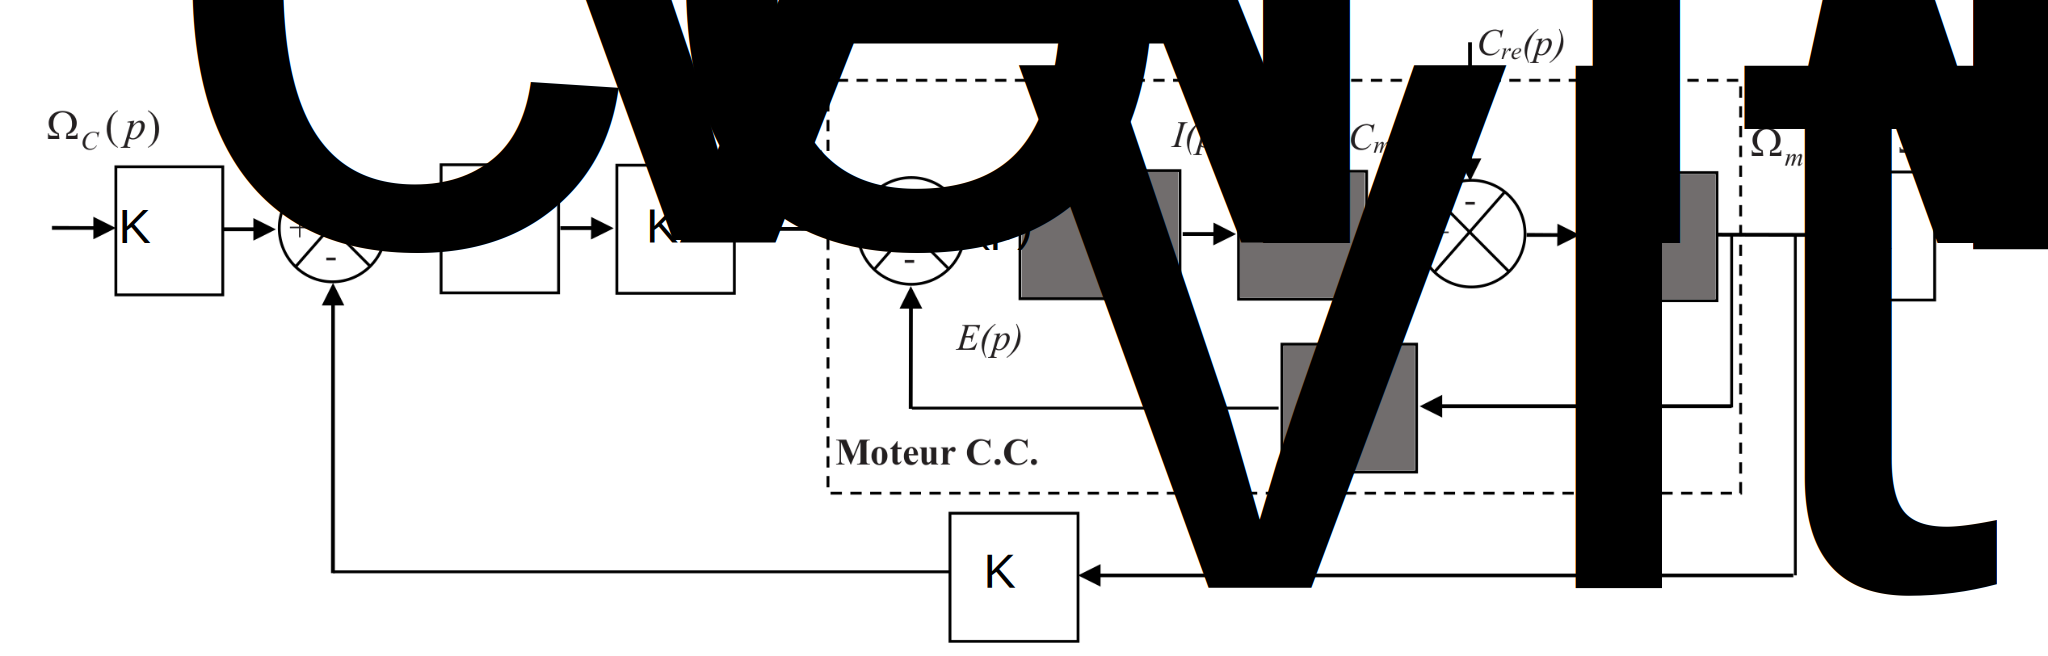
\includegraphics[width=0.9\linewidth]{img/DR02}
\end{center}}{
\begin{center}
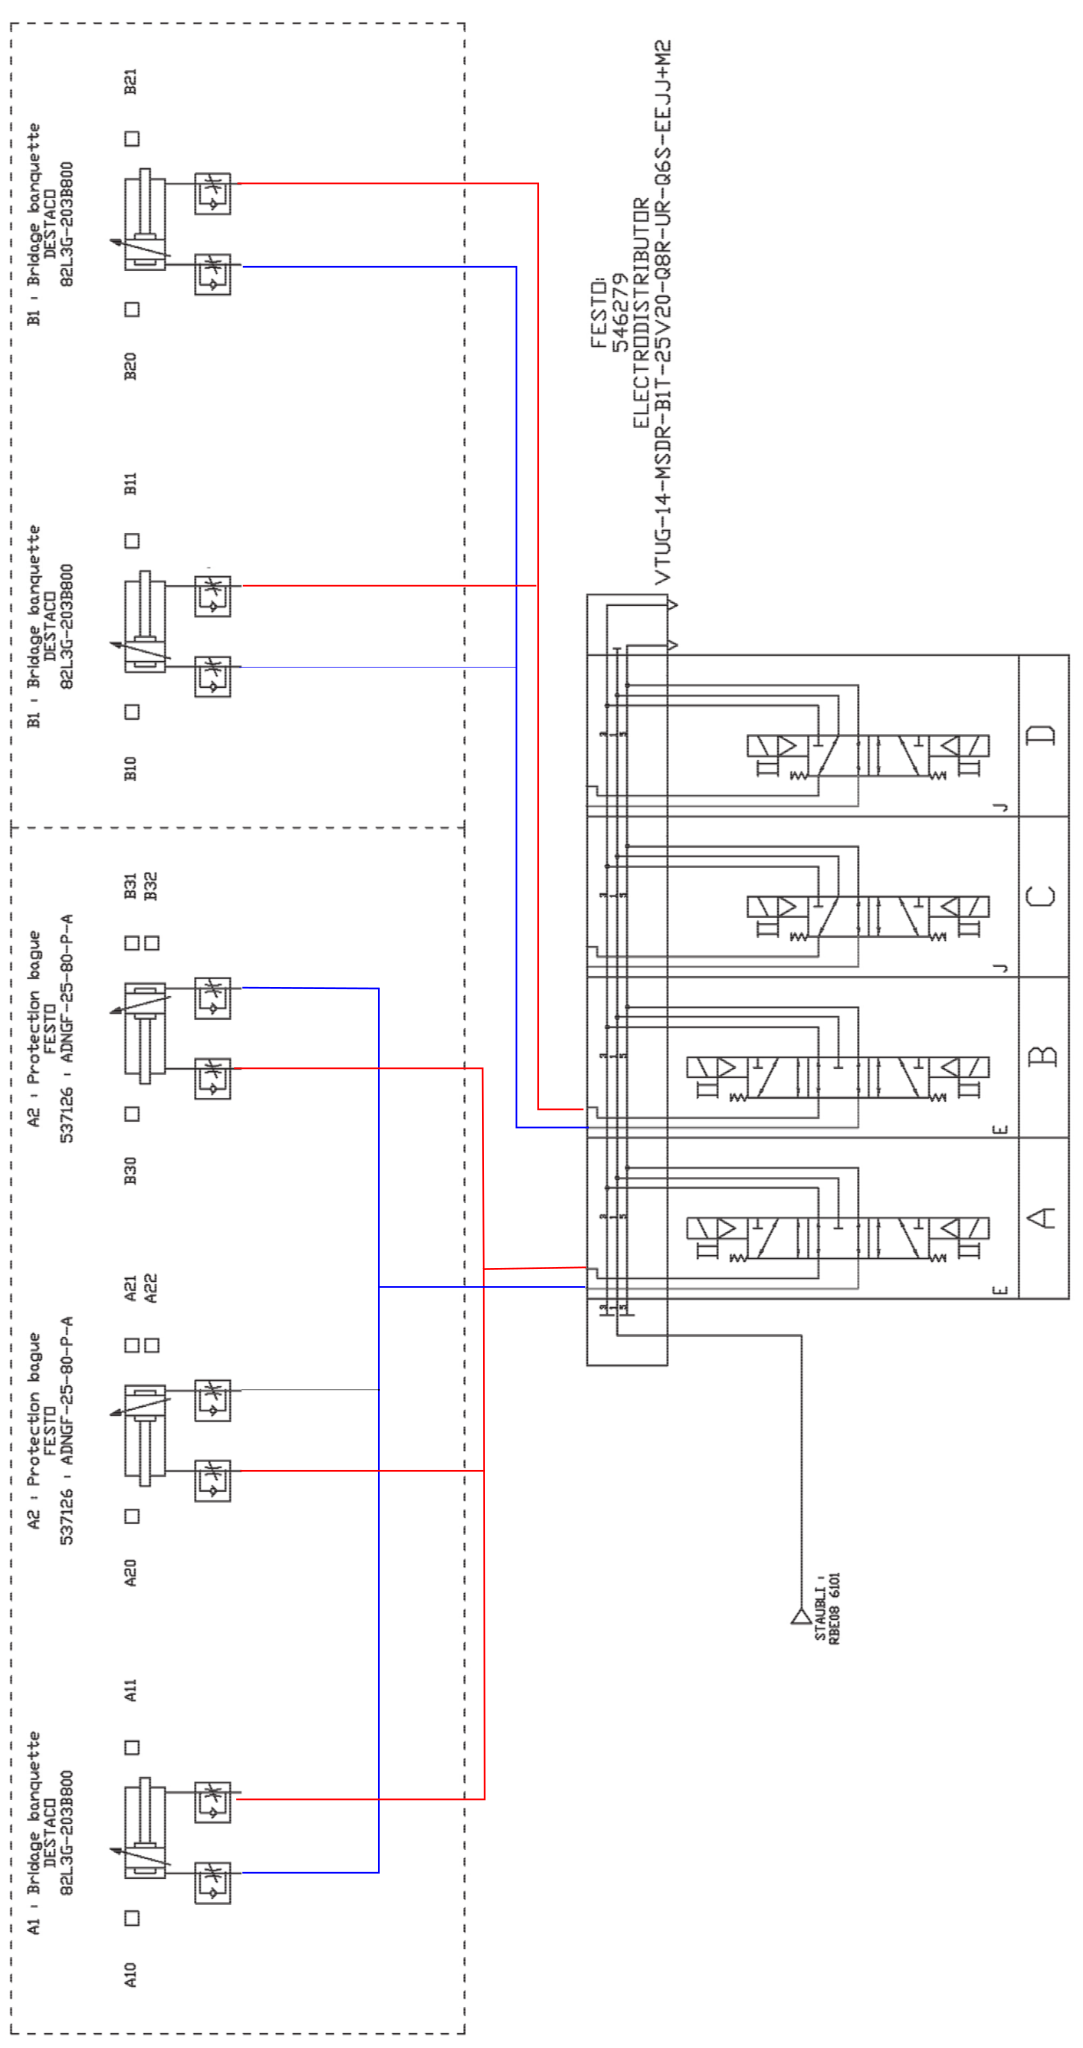
\includegraphics[width=0.9\linewidth]{img/DR02_cor}
\end{center}}

%3
\reponse{3}{}{
$V_{max}=\omega_mk_rr=3000\frac{2\pi}{60}\dfrac{1}{40}0,15=1,18m\cdot s^{-1}>1,1m\cdot s^{-1}$.

L'exigence 1.5.2 est donc vérifiée.
}

%4
\reponse{3}{}{
La distance D correspond à l'aire sous la courbe.

$D=\dfrac{V_{max}\delta t}{2}+V_{max}(T-2\delta t)+\dfrac{V_{max}\delta t}{2}=V_{max}(T-\delta t)$

Donc, $\delta t=T-\dfrac{D}{V_{max}}=0,91s$.}

\ifdef{\public}{\newpage}

%5
\reponse{7}{}{
A partir des équations du moteur, on obtient:
$u_m(t)=\dfrac{R_mJ}{2k_mk_t}\dfrac{dv(t)}{dt}+\dfrac{k_m}{k_t}v(t)$

$v(t)=\alpha_0\left(t-\tau_m+\tau_m e^{\frac{-t}{\tau_m}}\right)$, donc $\dfrac{dv(t)}{dt}=\alpha_0\left(1-e^{\frac{-t}{\tau_m}}\right)$

En remplaçant dans l'équation précédente on obtient:

$\frac{u_0}{\delta t}t=\dfrac{R_mJ}{2k_mk_t}\alpha_0\left(1-e^{\frac{-t}{\tau_m}}\right)+\dfrac{k_m}{k_t}\alpha_0\left(t-\tau_m+\tau_m e^{\frac{-t}{\tau_m}}\right)$


$\dfrac{k_m}{k_t}\alpha_0t-\frac{u_0}{\delta t}t+\dfrac{R_mJ}{2k_mk_t}\alpha_0\left(1-e^{\frac{-t}{\tau_m}}\right)-\dfrac{k_m}{k_t}\alpha_0\tau_m\left(1-e^{\frac{-t}{\tau_m}}\right)=0$

Donc, $\dfrac{k_m}{k_t}\alpha_0=\frac{u_0}{\delta t}$ et $\dfrac{R_mJ}{2k_mk_t}\alpha_0=\dfrac{k_m}{k_t}\alpha_0\tau_m$

Donc, $\alpha_0=\frac{u_0k_t}{\delta tk_m}$ et $\tau_m=\dfrac{R_mJ}{2k_m^2}$.
}

%6
\reponse{2}{
\vspace{-1cm}
\begin{center}
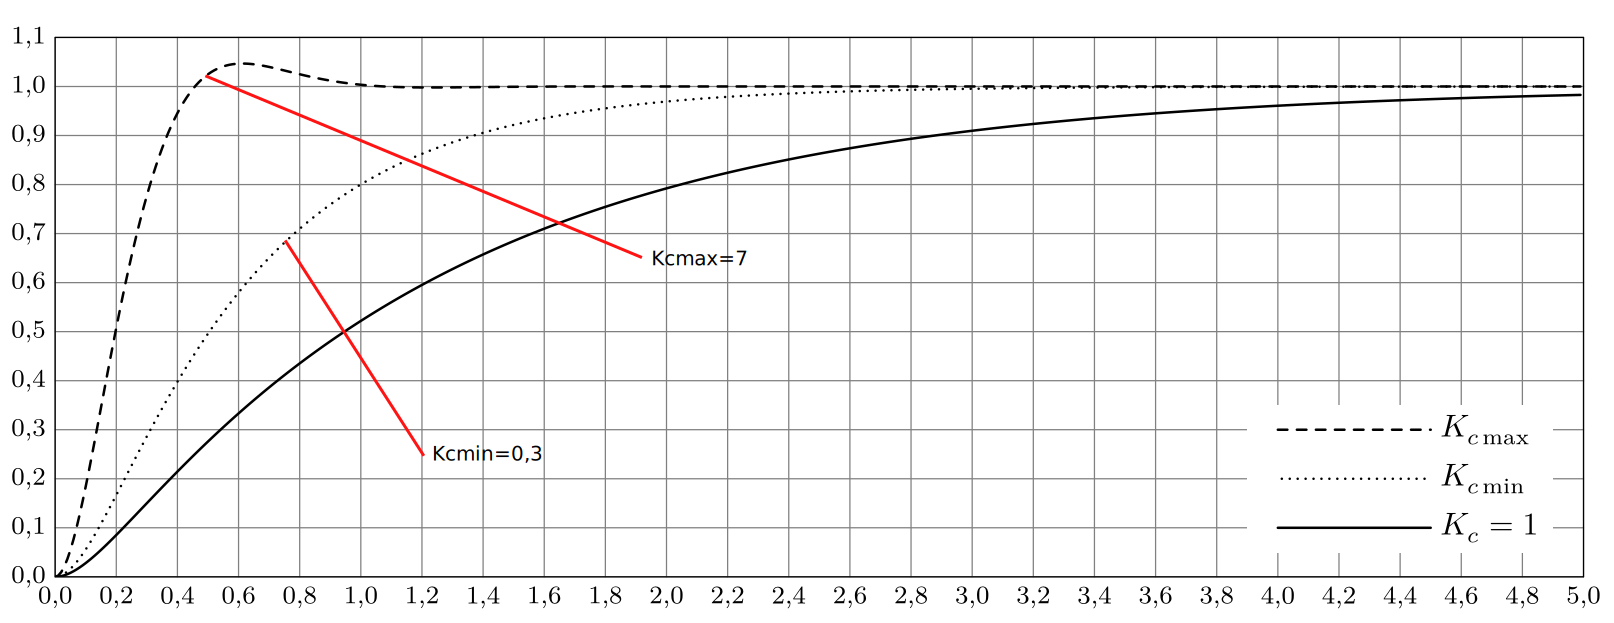
\includegraphics[width=0.4\linewidth]{img/DR06}
\end{center}
\vspace{-0.5cm}}{
\begin{center}
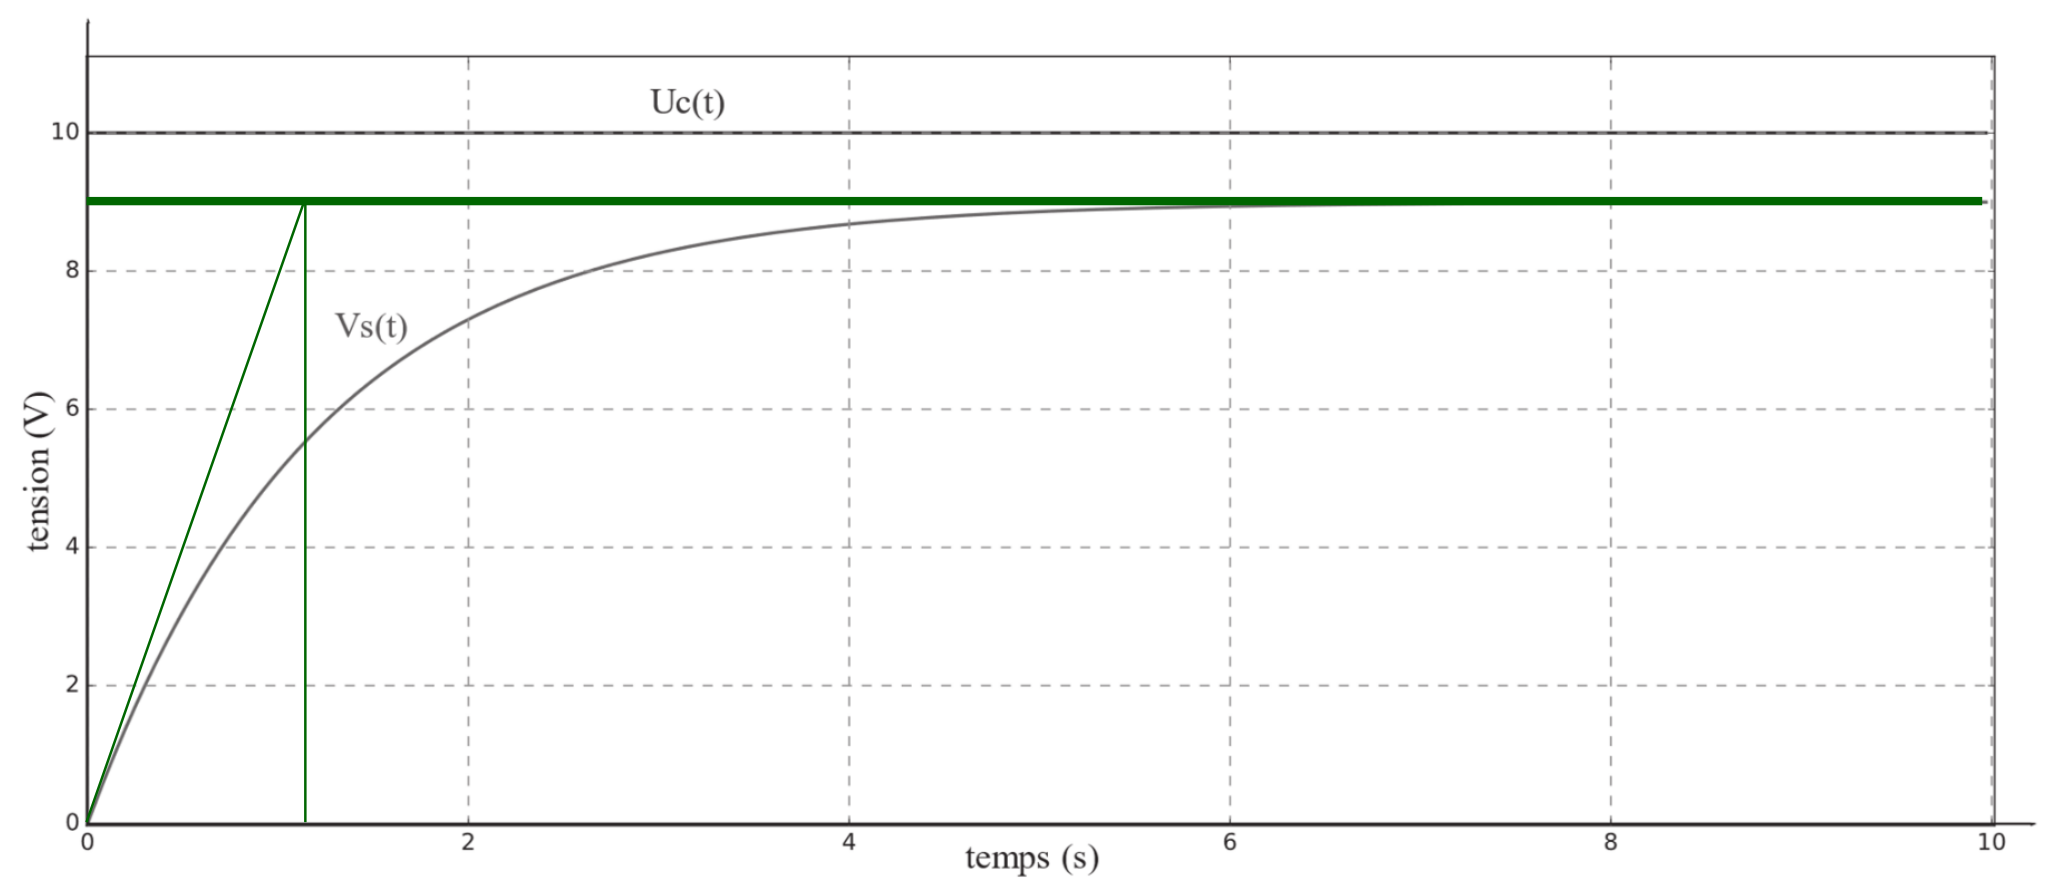
\includegraphics[width=0.4\linewidth]{img/DR06_cor}
\end{center}

Quand $t\rightarrow+\infty$, $v(t)$ tend vers une droite d'équation
$v(t)=\alpha_0(t-\tau_m)$.

Ainsi, $\tau_m=0,1s$.
}

%7
\reponse{4}{}{
En passant dans Laplace avec les CI nulles:\\
$U_m(p)=R_mI_m(p)+k_m\Omega_m(p)$\\
$2C_m(p)-C_r(p)=Jp\Omega_m(p)$\\
$C_m(p)=k_mI_m(p)$.

On a alors:
$H_m(p)=\dfrac{\dfrac{1}{k_m}}{\dfrac{R_mJ}{2k_m^2}p+1}$ et $H_r(p)=-\dfrac{\dfrac{R_m}{2k_m^2}}{\dfrac{R_mJ}{2k_m^2}p+1}$.}

\ifdef{\public}{\newpage}

%8
\reponse{1}{
\vspace{-1cm}
\begin{center}
\includegraphics[width=0.7\linewidth]{img/DR08}
\end{center}
\vspace{-0.5cm}}{
\begin{center}
\includegraphics[width=0.7\linewidth]{img/DR08_cor}
\end{center}
$K_c=628inc/tr=\frac{628}{2\pi}inc/rad$, soit $k_c\approx100 inc/rad$.

$\varepsilon(t)=0$ lorsque $v(t)=v_c(t)$, donc $k_a=\frac{K_c}{k_t}$.}

%9
\reponse{3}{}{
$C(p)=K_p\dfrac{1+\tau_ip}{\tau_ip}$ est un correcteur PI (Proportionnel-Intégral).Il augmente la classe de la FTBO de 0 à 1 cela augmente la précision de la réponse à un échelon.}

%10
\reponse{5}{}{
Comme $\tau_i=\tau_m$, $FTBO(p)=\dfrac{K_mK_cK_p}{\tau_mp}$

La FTBF a un retour unitaire, donc:

$FTBF(p)=\dfrac{\dfrac{K_mK_cK_p}{\tau_mp}}{1+\dfrac{K_mK_cK_p}{\tau_mp}}=\dfrac{1}{1+\dfrac{\tau_mp}{K_mK_cK_p}}$

$t_{r5\%}=\dfrac{3\tau_m}{K_pK_mK_c}=0,3$, donc $K_p=\dfrac{10\tau_m}{K_mK_c}=0,002$
}

%11
\reponse{1}{
\vspace{-1cm}
\begin{center}
\includegraphics[width=0.2\linewidth]{img/DR11}
\end{center}
\vspace{-0.5cm}}{
\begin{center}
\includegraphics[width=0.2\linewidth]{img/DR11_cor}
\end{center}

Le seuil présent dans la zone entourée représente des frottements secs. La perturbation a donc été prise en compte. La présence d'une perturbation montre qu'il est nécessaire de mettre en place un asservissement.
}

%12
\reponse{3}{
\vspace{-1cm}
\begin{center}
\includegraphics[width=0.5\linewidth]{img/DR13}
\end{center}
\vspace{-0.6cm}}{
\begin{center}
\includegraphics[width=0.5\linewidth]{img/DR13_cor}
\end{center}

Pour $0\leq t\leq \delta t$, $\dfrac{dv(t)}{dt}=\dfrac{V_{max}}{\delta_t}$, donc 
$C_m=r_{eq}(M_{eq}\dfrac{V_{max}}{\delta t}+F_{r,eq})=0,66Nm$

Pour $\delta t\leq t\leq T -\delta t$, $v(t)=V_{max}$, donc 
$C_m=C_0=r_{eq}F_{r,eq}=0,4Nm$

Pour $T-\delta t\leq t\leq T$, $\dfrac{dv(t)}{dt}=-\dfrac{V_{max}}{\delta_t}$, donc 
$C_m=r_{eq}(-M_{eq}\dfrac{V_{max}}{\delta t}+F_{r,eq})=0,136Nm$
}


%13
\reponse{3}{}{
On reprend les équations (1) et (3) : $u_m(t)=R_mi_m(t)+k_m\omega_m(t)$ et $C_m(t)=k_mi_m(t)$.

Soit $C_m(t)=\dfrac{k_m}{R_m}u_m(t)-\dfrac{k_m^2}{R_m}\omega_m(t)$

Le couple moteur est maximal au démarrage, il vaut $C_{max}=\dfrac{k_m}{R_m}u_m(t)$.

Avec $u_m(t)=100V$, on trouve $C_{max}=20Nm>>0,66Nm$ (Question 12).
}

%14
\reponse{3}{}{
$\vec{V}(A'\in g/0)=\vec{V}(O\in g/0)+\vec{A'O}\wedge\vec{\Omega}(g/0)=\vec{V}(O\in 1/0)+\vec{A'O}\wedge(\vec{\Omega}(g/1)+\vec{\Omega}(1/0))$.

$\vec{V}(A'\in g/0)=V\vec{y_1}+(r\vec{z}+e\vec{x_1})\wedge(\omega_g\vec{x_1}+\dot{\theta}\vec{z})$

$\vec{V}(A'\in g/0)=(V+r\omega_g-e\dot{\theta})\vec{y_1}$

De même, $\vec{V}(B'\in d/0)=(V+r\omega_d+e\dot{\theta})\vec{y_1}$
}

%15
\reponse{3}{}{

Roulement sans glissement en A' et en B' donc $\vec{V}(A'\in g/0)=\vec{0}$ et  $\vec{V}(B'\in d/0)=\vec{0}$, donc : \\
$V+r\omega_g-e\dot{\theta}=0$ et $V+r\omega_d+e\dot{\theta}=0$.

Donc, $r(\omega_g-\omega_d)-2e\dot{\theta}=0$ et $2V+r(\omega_g+\omega_d)=0$

Donc, $\dot{\theta}=\dfrac{r}{2e}(\omega_g-\omega_d)$ et $V=-\dfrac{r}{2}(\omega_g+\omega_d)$

Donc $C_1=\dfrac{r}{2e}$ et $C_2=-\dfrac{r}{2}$.
}

\ifdef{\public}{\newpage}

%16
\reponse{0}{
\begin{center}
\resizebox{0.6\textwidth}{!}{\begin{tabular}{|c|c|c|c|c|}
\hline
Mouvement & $V$ & $\dot{\theta}$ & $\omega_g$ & $\omega_d$ \\
\hline
Avant & $V_c$ & 0 &  & \\
\hline
Arrière & $-V_c$ & 0 &  & \\
\hline
Gauche & 0 & $\omega_c$ &  & \\
\hline
Droite & 0 & $-\omega_c$ &  & \\
\hline
\end{tabular}}
\end{center}}{\begin{center}
\resizebox{0.6\textwidth}{!}{\begin{tabular}{|c|c|c|c|c|}
\hline
Mouvement & $V$ & $\dot{\theta}$ & $\omega_g$ & $\omega_d$ \\
\hline
Avant & $V_c$ & 0 & $-\frac{V_c}{2C_2}$ & $-\frac{V_c}{2C_2}$ \\
\hline
Arrière & $-V_c$ & 0 & $\frac{V_c}{2C_2}$ & $\frac{V_c}{2C_2}$ \\
\hline
Gauche & 0 & $\omega_c$ & $-\frac{2\omega_c}{C_1}$ & $\frac{2\omega_c}{C_1}$\\
\hline
Droite & 0 & $-\omega_c$ & $\frac{2\omega_c}{C_1}$ & $-\frac{2\omega_c}{C_1}$\\
\hline
\end{tabular}}
\end{center}
}

%17
\reponse{3}{}{
On aurait pu utiliser un mécanisme à Croix de Malte à 6 branches, ou un moteur pas à pas.
}

%18
\reponse{5}{}{
Le moteur $M_1$ permet le rapprochement des mains (il agit sur l'engrenage pignon-crémaillère).

Le moteur $M_2$ permet le levage des pots.

Le guidage des mains par rapport au châssis est assuré par un mécanisme à 4 barres (parallélogramme): on a alors un mouvement de translation.
}

%19
\reponse{5}{}{
$h=m-N_c+6\mu$ avec:
\begin{itemize}
 \item  $m=1$ (1 mobilité utile, la translation sur $\vec{x}$, et aucune mobilité interne),
 \item $N_c=8$ (4 pivots glissants),
 \item $\mu=3$ (4 liaisons – 2 solides +1)
\end{itemize}

D'où $h=11$ très hyperstatique, ce qui apporte de la rigidité au mécanisme mais aussi des problématiques d'assemblage.
}

\ifdef{\public}{\newpage}

%20
\reponse{5}{}{

\begin{center}
\includegraphics[width=0.2\linewidth]{img/DR22_cor}
\end{center}

Les liaisons $S_0/S_1$ et $S_3/S_1$ peuvent être remplacées par des rotules

On a alors 1 mobilité utile + 1 mobilité interne, et 8 inconnues cinématiques (2 pivots + 2 sphériques)

Soit $h=m-N_c+6\mu=2-8+6.1=0$ isostatique.
}

%21
\reponse{5}{}{
On isole le pot, soumis aux actions mécaniques suivantes :
Action de pesanteur $\vec{P}=-mg\vec{z}$.

$\left\{T_{main1\rightarrow pot}\right\}=\left\{\begin{array}{c}
N_1\vec{x}+T_1\vec{z} \\\vec{0}\end{array}\right\}_{I_1}$

$\left\{T_{main2\rightarrow pot}\right\}=\left\{\begin{array}{c}
-N_2\vec{x}+T_2\vec{z} \\\vec{0}\end{array}\right\}_{I_2}$

On applique alors le théorème de la résultante statique au pot en équilibre, en projection sur $\vec{x}$ et $\vec{z}$ :

On a donc: $N_1-N_2=0$ et $T_1+T_2-mg=0$.

On se place à la limite du glissement : $T_1=f_pN_1$ et $T_2=f_pN_2$.

On obtient alors $N_1=N_2=\dfrac{mg}{2f_p}$.
}

%22
\reponse{4}{}{
Isoler le pignon. BAM: couple $C_0$ et actions des 2 crémaillères en
$I_{c1}(-F_{c1}\vec{x})$ et $I_{c2}(F_{c2}\vec{x})$.

Théorème de la résultante statique: $F_{c1}=F_{c2}$.

Le théorème du moment statique en $O$ sur $\vec{y}$: $C_0=2r_pF_{c1}$.
}

%23
\reponse{4}{}{
Théorème de la résultante statique sur $\vec{x}$: $F_{c1}-N_1=0$.

Donc, $C_0=2r_pF_{c1}=2r_pN_1=r_p\dfrac{mg}{f_p}$.

Donc, $r_0=\dfrac{r_p}{f_p}$ et ainsi $C_0=10,6 Nm< 12Nm$ donc le moteur retenu est donc satisfaisant.
}

%24
\reponse{3}{}{
La situation la plus défavorable est celle de la figure \ref{fig15} car le bras est tendu et porte un pot et aucun pot n'est chargé sur le robot ce qui aurait tendance à le lester pour éviter son basculement.
}

%25
\reponse{4}{}{
Isoler \{robot + pot\}. BAM: pesanteur et contact avec le sol.

Théorème du moment statique en D sur $\vec{x}$:

$-bN_c+(b-a)\dfrac{Mg}{2}-c\dfrac{mg}{2}=0$ d'où : $N_c=\dfrac{(b-a)Mg-cmg}{2b}$
}

%26
\reponse{3}{}{
On obtient alors $m=\dfrac{b-a}{c}M=22,5kg$ l'exigence 1.5.3 est donc validée.
}

\ifdef{\public}{\newpage}

%27
\reponse{0}{
\begin{center}
\includegraphics[angle=90,width=0.9\linewidth]{img/Pince Robot ASEA}
\end{center}}{
\begin{center}
\includegraphics[width=\linewidth]{img/Pince Robot ASEA_cor}
\end{center}
}

\end{document}

%27
\reponse{3}{}{
Les équations (5) et (6) correspondent à l'application du théorème de la résultante dynamique au robot en mouvement par rapport au référentiel galiléen $R_0$, au point D, projeté sur $\vec{y}$ et $\vec{z}$.

L'équation (7) correspond à l'application du théorème du moment dynamique au robot en mouvement par rapport au référentiel galiléen $R_0$, projeté sur $\vec{x}$, au point D.
}

%28
\reponse{3}{}{
En isolant la roue avant et en appliquant le théorème du moment dynamique en son centre, il vient immédiatement $C_{mr}-rT_D=0$ (moment d'inertie de la roue négligée).

D'où $T_D=\dfrac{C_{mr}}{r}$.
}


%29
\reponse{3}{}{
Seule la roue avant étant motrice, je suppose $T_C=0$ (ce qui peut se justifier par l'application du PFD à la roue arrière (inertie négligée), en son centre)

La relation (5) donne alors $T_D=\dfrac{M}{2}\gamma$,  AN : $T_D=33N$

D'autre part, les équations (6) et (7) permettent d'écrire :
$N_C=(b-a)\dfrac{M}{2b}g+h\dfrac{M}{2b}\gamma$ soit $N_D=\dfrac{M}{2}g-(b-a)\dfrac{M}{2b}g-h\dfrac{M}{2b}\gamma=\dfrac{M}{2b}(ag-h\gamma)$.

AN : $N_D=178N$

On calcule alors $\dfrac{T_D}{N_D}= 0,18<f$ il y a donc adhérence (roulement sans glissement).
}


%30
\reponse{0}{}{
A la limite du glissement, $T_D=\dfrac{M}{2}\gamma_{max}=fN_D$

Soit $\gamma_{max}=\dfrac{2fN_D}{M}$ AN : $\gamma_{max}=2,97m\cdots^{-2}$

Dans ces conditions, la durée de la phase d'accélération pour atteindre $V_{max}=1,1m\cdots^{-1}$ (exigence 1.5.2) vaut $t_{acc}=\dfrac{V_{max}}{\gamma_{max}}=0,37s$.
}


\end{document}
